\documentclass[../thesis.tex]{subfiles}

\begin{document}

\section{Ý tưởng cơ bản}

Một ý tưởng về một layer off-chain đã xuất hiện từ lâu trong cộng đồng, ý tưởng chính là thay vì thực hiện các giao dịch với các phép tính phức tạp bên trong 
blockchain network, người ta thực hiện các giao dịch đó bên ngoài blockchain, sau đó bằng một cách nào đó người ta đảm bảo rằng các giao dịch đó là hợp lệ. Người dùng có thể gửi các tài sản số vào các layer này, thực hiện tính toán và rút các tài sản này ra khi cần thiết.

Bằng cách này chi phí thực thi một giao dịch trong Ethereum giảm đi đáng kể, nhưng câu hỏi đặc ra là làm sao ta đảm bảo được cách chúng ta thực hiện các giao dịch là đúng? Thật tuyệt vời zk-SNARK gần như là một công cụ hoàn hảo để làm điều này. Trong mỗi giao dịch ta sinh ra một bằng chứng cho giao dịch đó sau đó gửi bằng chứng đó lên blockchain network, network sẽ có một smart contract có thể kiểm chứng bằng chứng có đúng hay không. Từ đó cập nhật trạng thái mới vào smart contract. 

Nhưng ta có thể làm tốt hơn nữa thay vì mỗi lần chỉ xử lý một giao dịch một lúc, tại sao ta không gộp nhiều transaction lại và sinh bằng chứng trong một lần. 
Ta gọi một tập transaction như vậy là batch. Ta cũng tiến hành nét dữ liệu trong batch lại để tiết kiệm chi phí hơn. Hơn nửa ta có thể dùng merkle tree để lưu lại trạng thái hiện tại của các account. Bài toán cần xác thực lúc này là kiểm tra việc cập nhật merkle tree. Việc dùng merkle tree ở đây giảm chi phí cho việc kiểm tra và cập nhật trạng thái rất nhiều, điều này tương đồng với cách các blockchain network dùng merkle tree để nét dữ liệu trong block thành merkle root vậy. Trên blockchain network, ta lưu giá trị của merkle root hash trên blockchain. Với một batch ta có thể kiểm chứng việc cập nhật trạng thái, tính toán merkle root mới và cập nhật lại merkle root lưu trên blockchain. Đây là ý tưởng cơ bản của zk rollup. 

\begin{figure}[ht]
   \centering
	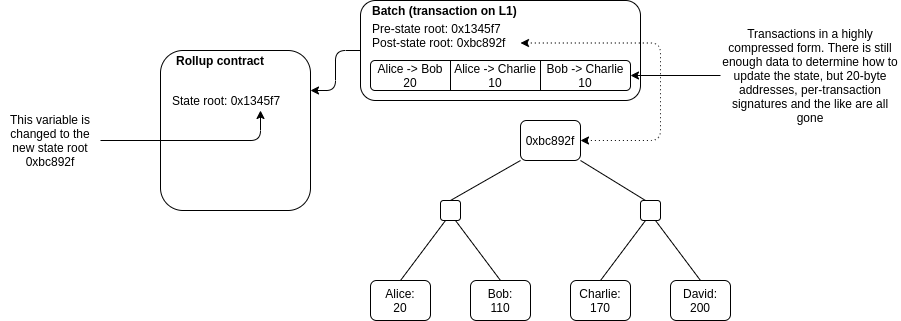
\includegraphics[width=1\textwidth]{diag2.png}
    \caption{Hình dáng cơ bản của một zk-Rollup layer \cite{vitalik}}
    \label{simple-rollup}
\end{figure}

\section{Kiến trúc zk-Rollup cho bài toán giao dịch token}
Ta đã nắm được ý tưởng cơ bản của zk-Rollup, giờ công việc tiếp theo sẽ là xây dựng một layer 2 dùng zk-Rollup. Trong layer của tôi, tôi chỉ cho phép giao dịch một loại token, hiển nhiên ta có thể mở rộng nó trong tương lai. Để cho dễ dàng triển khai thuật toán ở đây tôi quy định hàm merkle\_verify(data) là hàm kiểm tra xem data đó có nằm trong merkle tree hay không. Hàm merkle\_update(data) là hàm cập nhật lại root merkle tree.

\subsubsection{Cấu trúc account}
Trong phần này ta xem xét tới cấu trúc của account leaf của merkle tree. Trong hình \ref{simple-rollup} ta đã thấy các nút lá của merkle tree lưu lại sẽ trạng thái của account. 
Trong trường hợp này tôi quy định trạng thái account sẽ có schema như sau:

\begin{minted}[fontsize=\footnotesize]{json}
{
	"layer_index": "chỉ số của account trong layer",
	"public_key_x": "public key",
	"public_key_y": "public key",
	"nonce": "số lượng transaction đã thực hiện",
	"balance": "số token trong tài khoản"
}
\end{minted}

Trong đó public\_key\_x, publickey\_y là khoá công khai của chữ ký số trong thuật toán EdDSA của tài khoản sở hữu layer\_index trong merkle tree, layer\_index cho biết số thứ tự của account, đồng thời cũng cho biết vị trí của account trong merkle tree của layer, balance là số tiền còn lại của account, nonce là số lượng giao dịch mà account đó đã thực hiện trên layer 2.

Ta có giá trị hash của nút leaf được tính như sau:

\begin{minted}{python}
leaf_hash = Hash(public_key_x, public_key_y, 
                 layer_index, balance, nonce)
\end{minted}

Trong đó ta có account có index bằng 0 là một index đặt biệt (Từ đây ta gọi nó là index zero). Nó đại diện cho chính smart contract của layer. Khi có token chuyển từ bên ngoài vào smart contract hay nói đúng hơn là quá trình deposit xảy xa. Ta sẽ quy ước có token chuyển từ index zero về index trong layer của account được tạo đó. Tương tự khi có lệnh withdraw, rút tiền từ layer về Ethereum account, bên trong layer ta quy ước sẽ chuyển token từ account đó về index zero của layer.

Ta cũng sử dụng chữ ký số ta bảo đảm mọi hành động thay đổi trạng thái điều xuất phát từ người có quyền trên account, mà không phải là một tác nhân xấu nào đó.
Điều này đảm bảo tính an toàn cho giao dịch.

\subsubsection{Cấu trúc transaction}
Với transaction ta có cấu trúc như sau.
\begin{minted}[fontsize=\footnotesize]{json}
{
	"sender": "layer index of sender",
	"receiver": "layer index of receiver",
	"amount": "amount",
	"sig":{ 
			"A", 
			"R", 
			"s"
  	 } 
}
\end{minted}
Trong đó sender, receiver lần lước là index của sender account, amount là số token bạn muốn gửi, sig là chữ ký của người gửi, để chứng thực cho hành động họ muốn thực hiện. Tuỳ theo loại transaction mà ta quy định các cơ chế riêng để xử lý chúng. Ở đây tôi sử dụng thuật toán chữ ký số EdDSA vì nó tương đối thân thiện với zk-SNARK.

\subsubsection{Cơ chế chứng minh giao dịch trong layer 2} 
Giờ ta xem xét cách mà ta thực hiện một transaction trong zk-Rollup. 
Giả sửa ta có một transaction mang theo nội dung mà ta quy định trong phần định dạng transaction như trên. Để sinh bằng chứng cho một giao dịch ta làm như sau:

\begin{enumerate}
\item Chứng minh nút sender chắc chắc thuộc về merkle tree bằng hàm merkle\_verify. 
\item Chứng minh chử ký khớp với chử ký người gửi. 
\item Giảm balance của sender.
\item Tăng nonce của sender.
\item Cập nhật merkle tree bằng merkle\_update, ta cũng nhận được một merkle root mới, ta gọi giá trị này là intermediate\_root. 
\item Chứng minh rằng receiver thuộc merkle tree bằng merkle\_verify.
\item Tăng balance của receiver.
\item Cập nhật lại merkle tree bằng merkle\_update với data của receiver và intermediate\_root, ta có được một merkle root mới gọi là final\_root.
\end{enumerate}

Khi muốn chứng minh một transaction mới ta làm điều tương sự, nhưng với final\_root ta vừa có được khi ta xử lý transaction trước đó. Các transaction trong patch sẽ gối đầu nhau, từ transaction đầu tiên đến transaction cuối cùng. Cuối cùng ta có được một bằng chứng, ta gửi bằng chứng này lên Ethereum, kiểm tra và thức hiện các phép tính cần thiết cho việc cập nhật.

\subsubsection{Cơ chế chứng minh một cho một giao dịch deposit hoặc withdraw}
Ta áp dụng cơ chế này khi có một người dùng muốn gửi token amount vào layer của chúng ta. Theo quy ước lúc này trong layer 2 sẽ có một transaction từ index zero tới account index của người gửi. Có 2 trường hợp xảy:

Trường hợp thứ nhất, tài khoản đã có sẳn trong layer. Ta chỉ cần thực hiện lệnh chuyển token vào layer và sinh ra bằng chứng về giao dịch đó. Trong trường hợp thứ 2 phức tạp hơn, người gửi chưa có trong layer. Ta cần tạo một account mới cho địa chỉ đó trên layer 2, và thực hiện tương tự trường hợp thứ nhất.

Đối với withdraw tuân theo quy ước ta thực hiện một transaction từ account index của người muốn rút tiền về index zero. 

\subsubsection{Tạo bằng chứng và xác minh transaction cho một batch}
Smart contract của layer 2 là nơi ta xác minh các giao dịch, cũng như gửi token ra - vào token trong trường hợp có lệnh gửi token hay rút token. Trong smart contract, ta lưu lại merkle root hiện của merkle tree trong layer. Mỗi khi cập nhật một batch ta tiến hành kiểm tra bài toán $Verify(merkle\_root,new\_merkle\_root, proof))$.


Nếu điều này là đúng, chứng tỏ các giao dịch trong bash đó điều chính xác. Ta gọi phương thức rollup của smart contract cho phép ta kiểm tra một batch có đúng hay không và cập nhật lại merkle\_root trong trường hợp mọi thứ điều hoạt động trơn chu. Lúc này Hàm rollup có các đối số đầu vào là proof(bằng chứng), new\_merkle\_root.

Thay vì lưu lại các trạng thái của account vào smart contract rồi sửa đôi chúng khi có một batch mới được gửi lên, tôi không lưu các trạng thái zk-rollup account vào contract  mà thay vào đó tôi đưa thông tin về các transaction vào đối số của hàm rollup. Để đảm bảo transaction data gửi lên là đúng tôi sẽ tạo thêm một bài toán đó là kiểm sha256(batch data) = batch\_hash. Tức là lúc đó bằng chứng phải thoả mãng bài toán.

\[
\begin{cases}
  Verify(merkle\_root,new\_merkle\_root, proof) = true \\
 	Verify(batch\_data, batch\_hash, proof) = true
\end{cases}
\]

Lúc đó hàm rollup có các đối số đầu vào là proof(bằng chứng), new\_merkle\_root và batch transaction data. Do ethereum lưu lại lịch sử giao dịch tức khi ta bị mất data base hay layer 2 không còn hoạt động nửa thì người dùng vẫn có thể lấy lại được lịch sử giao dịch từ đó có thể tự tạo bằng chứng và rút tiền về layer 1.

\section{Xây dựng layer 2 dùng zk-Rollup}
\subsection{Môi trường phát triển}
Với mục đích thử nghiệm, chúng tôi chọn bộ toolkit ethsnarks\cite{ethsnark} được viết bằng c++, python, javascript và solidity. Ethsnarks cung cấp các công cụ cho việc xây dựng một hệ thống zk-snark dễ dàng hơn. Chi tiết về ethsnark bạn có thể tham khảo trong link ở phần tham khảo. Ngoài ra chúng tôi còn sử dụng hardhat là một bộ công cụ cho phép tạo testnet, viết và kiểm thử smart contract trong Ethereum. 
Sử dụng phần cứng có thông số như bảng bên dưới.
\begin{table}[H]
\centering
\begin{tabular}{|l|l|}
\hline
CPU & 2.9 GHz Dual-Core Intel Core i5 \\ \hline
RAM &  8 GB 1867 MHz DDR3\\ \hline
SSD &  128G\\ \hline
OS &  macOS\\ \hline
\end{tabular}
\caption{Thông tin phần cứng}
\label{tab:my-table}
\end{table}

\subsection{Các thành phần cơ bản}
Ứng dụng được viết dưới dạng dòng lệnh, gồm 2 thành phần: 
\begin{itemize}
\item Prover chịu trách nhiệm sinh ra bằng chứng từ các transaction đầu vào.
\item Smart contract chịu trách nhiệm kiểm tra bằng chứng được cung cấp từ phía prover và cập nhật trạng thái mới cho hợp đồng.
\end{itemize}

\section{Kết quả thực nghiệm}
Phần này trình bày kết quả thực nghiệm với các kịch bản sau:

Merkle tree cho layer này có độ sâu 8(chứa được $2^8=256$ account). Ta tạo 10 account cho layer, sau đó thực hiện các lệnh deposit từ 10 account này, tiếp theo thực hiện lệnh transfer token ngẩu nhiên bên trong layer, cuối cùng rút hết token từ trong layer về địa chỉ Ethereum của các account. Ở đây tôi không tính chi phí cho tạo account trên layer 2.

Dưới đây là bảng chi phí gas lần lược cho các trường hợp số transaction cho mỗi batch lần lược là 25, 30, 35, 40 và 50.

\begin{table}[H]
\centering
\begin{tabular}{|l|l|l|l|l|}
\hline
 Transaction pre batch & deposit &  transfer & withdraw  \\ \hline
25 & 609174 &  310640 & 419953  \\ \hline
30 & 661589 &  314477& 434960  \\ \hline
35 & 690985 & 318637 & 427774  \\ \hline
40 & 731896 & 322582 & 431625 \\ \hline
50 & 813623 & 322582 & 428217 \\ \hline

\end{tabular}
\caption{Chi phí gas với các kích thước batch khác nhau}
\label{tab:my-table}
\end{table}

Nếu không dùng zk-Rollup, gas của một transaction là khoảng 31000 gas. Suy ra số gas cần tiêu thụ cho việc chuyển token là 30 * 31000 = 930000 gas. Trong khi sử dụng zk-Rollup, nếu ta chỉ thực hiện các giao dịch bên số gas tiêu thụ chỉ là 314477. Suy ra trung bình chi phí cho mỗi giao dịch là 10482 gas. Thấp hơn rất nhiều so với chi phí phải chịu khi thực hiện giao dịch trực tiếp trên Ethereum.

Hơn nữa trong zk-Rollup chi phí tốn cho việc verify là vào khoảng 290000, suy ra gas tiêu tốn cho 30 transaction là 314477 - 290000 = 24477. Lấy con số này chia cho 30, thì mỗi người chỉ chịu khoảng 818 tức là gần 1000 gas cho việc chuyển token. Với gas block limit hiện tại là 15 triệu suy ra số transaction có thể thực hiện là (15000000 - 290000) / 1000 = 14710 transaction. Hiển nhiên các tính toán này được xem xét trong các điều kiện tối ưu. 
Thực tế tuy không đạt được kết quả hoàn hảo như vậy nhưng cũng đem lại kết quả rất khả quan. 


\end{document}
